%!TEX root = ../dissertation.tex

\hypertarget{(chap:capitolo4)}{}
\chapter{Modelli per il Bin Packing}
In questo capitolo presenteremo prima una rapida introduzione ai modelli matematici, tratta dal \bit{libro}{ricerca}, per poi analizzare nel dettaglio ciascun modello utilizzato spiegando ciascun vincolo e delineandone quindi l'idea di base.
\section{Modelli di programmazione matematica}
Quando si parla di problemi di ottimizzazione spesso si fa riferimento alla ricerca operativa e ai modelli matematici. Questi modelli producono una soluzione che massimizza o minimizza una funzione obiettivo $f ( x ) $ su un certo dominio, questa funzione può rappresentare un aspetto di costo o guadagno. I polinomi lineari $g_{i} (x)$. 		 
La soluzione restituita ha la proprietà di essere una soluzione ottima. La funzione obiettivo solitamente viene rappresentata come segue:
$$ max\; z = f ( x )\;\; (oppure\; min\; z = f ( x ))$$
s.t.
$$g_i (x) = \begin{cases} \leq b_i \\ = b_i, & i = 1,\dots,m \\ \geq b_i \end{cases}$$
$$x = (x_1,\dots,x_n) \in X \subseteq \mathbb{R}^n$$
Dove $g_i$ è una matrice $m \cdot n$ con vettori riga: $g_1,\dots,g_m$ e $b_i$ è un vettore in $\mathbb{R}^{m}$
In un modello sono presenti:
\begin{itemize}
	\item \textbf{Variabili decisionali}: sono variabili con un dominio prefissato, che vengono utilizzate per formulare tutti gli altri elementi del modello, agendo sui valori assunti dalle stesse si troverà la soluzione ottima;
	\item \textbf{Funzione obiettivo}: funzione che deve essere massimizzata o minimizzata in base agli altri elementi su un dominio dato;
	\item \textbf{Vincoli}: serie di vincoli che correlano tra loro le variabili decisionali e permettono di descrivere condizioni fisiche o requisiti particolari richiesti dalla soluzione.
\end{itemize}
\section{Modelli di programmazione lineare}
Particolari tipi di problemi di programmazione matematica sono quelli in cui la funzione obiettivo $f(x)$ e i vincoli $g_i(x)$ sono funzioni lineari, in tal caso si può parlare di modello di \textit{programmazione lineare}, espresso nel seguente modo:
$$ max\; z = \sum_{j=1}^n c_j x_j $$
s.t.
$$\sum_{j=1}^n a_{ij} x_j = \begin{cases} \leq b_i \\ = b_i, & i = 1,\dots,m \\ \geq b_i \end{cases}$$
$$x = (x_1,\dots,x_n) \in X \subseteq \mathbb{R}^n$$
Nonostante i modelli non lineari siano a volte molto più compatti ed intuitivi da capire, i modelli lineari mantengono comunque semplicità e sono facilmente risolvibili. Sono molti gli strumenti ad uso \glo{commerciale} e \glo{open source} disponibili per la loro risoluzione. Quello utilizzato durante lo stage è il \glo{solver} open source di programmazione lineare intera \bit{Cbc}{cbc} scritto in \bit{C++}{cpp} interfacciato con \bit{Python}{python} grazie a \bit{Google Or-Tools}{ortools}. La creazione di un modello lineare parte dall'osservazione di un problema reale, fissando un obiettivo e creando vincoli che descrivano i requisiti estratti dal problema astraendo il tutto ad un insieme di vincoli lineari.
Ogni variabile può avere un dominio differente, continua ($x_j \in \mathbb{R}$), intera positiva ($x_j \in \mathbb{Z}^+$) o binaria ($x_j \in \{0,1\}$) a seconda dell'utilizzo che se ne deve fare.
\section{Big M}
Le Big M, valori opportunamenti definiti che permettono di attivare o disattivare alcuni vincoli, sono state definite cercando di assegnargli un valore come segue:
\begin{itemize}
	\item M: dato gli n oggetti, M è la somma della massima dimensione tra $w_i$ e $d_i$ dell'oggetto i-esimo;
	\item $M_w$: viene definito come la larghezza del camion W sommato ad M;
	\item $M_d$: viene definito come la lunghezza del camion D sommato ad M.
\end{itemize}

\section{Modello 2D}
Il modello per la versione 2D è stato preso dall'\bit{articolo}{modello}, esso considera solo larghezza e profondità degli oggetti e non ne permette la rotazione. L'idea di base è quella di considerare solo la \textit{visione aerea} del contenitore che viene così approssimata ad un rettangolo. Questo rettangolo ha larghezza prefissata e profondità infinita, le due dimensioni posso essere considerate come assi di un piano cartesiano aventi origine nel punto di intersezione tra i due assi, individuato nella figura \eqref{fig:veduta_aerea} dal pallino verde, per convenzione diciamo che l'asse x sarà quello della larghezza e l'asse y quello della profondità.
\begin{figure}[H]
	\begin{center} 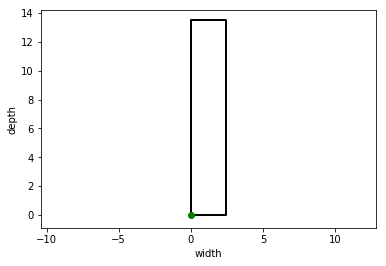
\includegraphics[scale=0.6]{figures/cartesian_wd}
		\caption[Veduta area - piano cartesiano]{Veduta area del container}  
		\label{fig:veduta_aerea}
	\end{center}
\end{figure}

\noindent Il modello consiste delle seguenti variabili continue positive:
\begin{itemize}
	\item la variabile continua $x_{i}$ con $i \in I$ individua la coordinata sull'asse x del vertice in basso a sinistra dell'oggetto i;
	\item la variabile continua $y_{i}$ con $i \in I$ individua la coordinata sull'asse y del vertice in basso a sinistra dell'oggetto i;
	\item la variabile continua $D$ rappresenta i metri lineari rispetto la profondità e va minimizzata.
\end{itemize}
Il modello consiste delle seguenti variabili binarie:
\begin{itemize}
	\item la variabile binaria $l_{ij}$ con $i,j \in I$ assume il valore 1 se l'oggetto i è situato alla sinistra dell'oggetto j, altrimenti è 0;
	\item la variabile binaria $b_{ij}$ con $i,j \in I$ assume il valore 1 se l'oggetto i è situato al di sotto dell'oggetto j, altrimenti è 0.
\end{itemize}

\begin{align}
	& \underset{}{\text{min D}} \label{equa10}\\
	  & \text{s.t.} &   & l_{ij} + l_{ji} + b_{ij} + b_{ji} \geq 1      & i < j    &   & i,j \in I \label{equa11} \\
	  &             &   & y_i - y_j + M_d b_{ij} \leq M_d - d_i         &          &   & i,j \in I \label{equa12} \\
	  &             &   & x_i - x_j + M_w l_{ij} \leq M_w - w_i         &          &   & i,j \in I \label{equa13} \\
	  &             &   & x_i + w_i \leq W                              &          &   & i \in I   \label{equa14} \\
	  &             &   & y_i + d_i \leq D                              &          &   & i \in I   \label{equa15} \\
	  &             &   & b_{ij}, l_{ij} \in \{0,1\}                    & i \neq j &   & i,j \in I \label{equa16} \\
	  &             &   & x_{i}, y_{i}, w_{i}, d_{i} \in \mathbb{R}^{+} &          &   & i \in I  \label{equa17}  
\end{align}

Spieghiamo ora il significato di ciascun vincolo:
\begin{itemize}
	\item il vincolo~\eqref{equa10} la funzione obiettivo minimizza i metri lineari rispetto alla profondità;
	\item il vincolo~\eqref{equa11} impone che presi due oggetti almeno uno dei due si trovi dietro o alla sinistra dell'altro;
	\item il vincolo~\eqref{equa12} dice che se $b_{ij} = 1$ allora impone che l'oggetto i si trovi dietro l'oggetto j, altrimenti il vincolo viene disattivato. 
	\item il vincolo~\eqref{equa13} dice che se $l_{ij} = 1$ allora impone che l'oggetto i si trovi alla sinistra l'oggetto j, altrimenti il vincolo viene disattivato. 
	\item il vincolo~\eqref{equa14} impone che dato il valore $x_i$, corrispondente alla coordinata x dell'angolo sinistro più arretrato dell'oggetto, sommandoci la larghezza $w_i$ dell'oggetto e ottenuta quindi la coordinata x dell'angolo destro più arretrato, questa sia contenuta nell'intervallo [0,W];
	\item il vincolo~\eqref{equa15} impone che dato il valore $y_i$, corrispondente alla coordinata y dell'angolo sinistro più arretrato dell'oggetto, sommandoci la profondità $d_i$ dell'oggetto e ottenuta quindi la coordinata y dell'angolo sinistro più avanzato, questa sia contenuta nell'intervallo [0,D];
\end{itemize}

\section{Modello 2D con rotazione}
Il modello 2D con rotazione introduce in più rispetto al modello 2D la rotazione degli oggetti rispetto la propria base come mostrato in figura~\eqref{fig:pacchi_ruotati}.
\begin{figure}[H]
	\begin{center} 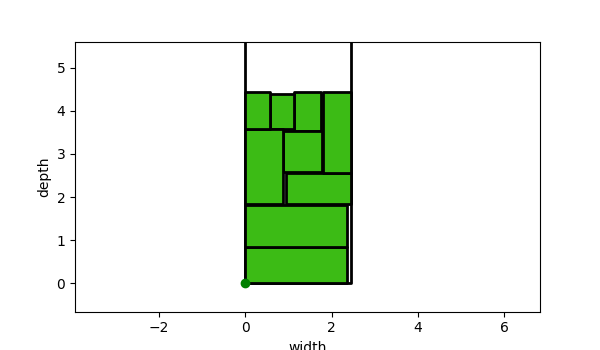
\includegraphics[scale=0.6]{figures/2dr}
		\caption[Pacchi ruotati]{Veduta aerea di 9 pacchi, alcuni ruotati.}
		\label{fig:pacchi_ruotati}
	\end{center}
\end{figure}

\noindent Il modello consiste delle seguenti variabili continue positive:
\begin{itemize}
	\item la variabile continua $x_{i}$ con $i \in I$ individua la coordinata sull'asse x del vertice in basso a sinistra dell'oggetto i;
	\item la variabile continua $y_{i}$ con $i \in I$ individua la coordinata sull'asse y del vertice in basso a sinistra dell'oggetto i;
	\item la variabile continua $D$ rappresenta i metri lineari rispetto la profondità e va minimizzata.
	\item la variabile continua $\Omega_{i}$ con $i \in I$ assume il valore $d_i$ se l'oggetto è stato ruotato altrimenti $w_i$;
	\item la variabile continua $\Delta_{i}$ con $i \in I$ assume il valore $w_i$ se l'oggetto è stato ruotato altrimenti $d_i$;
\end{itemize}
Il modello consiste delle seguenti variabili binarie:
\begin{itemize}
	\item la variabile binaria $l_{ij}$ con $i,j \in I$ assume il valore 1 se l'oggetto i è situato alla sinistra dell'oggetto j, altrimenti è 0;
	\item la variabile binaria $b_{ij}$ con $i,j \in I$ assume il valore 1 se l'oggetto i è situato al di sotto dell'oggetto j, altrimenti è 0.
	\item la variabile binaria $r_{i}$ con $i \in I$ assume il valore 1 se l'oggetto i è ruotato rispetto la propria base di 90°, ne risulta che $w_{i}$ e $d_{i}$ sono invertiti, altrimenti 0;
\end{itemize}

\begin{align}
	& \underset{}{\text{min D}}\\
	  & \text{s.t.} &   & l_{ij} + l_{ji} + b_{ij} + b_{ji} \geq 1                              & i < j    &   & i,j \in I \label{equa21} \\
	  &             &   & \Delta_i = d_i (1 - r_i) - w_i r_i                                    &          &   & i,j \in I \label{equa22} \\
	  &             &   & \Omega_i = w_i (1 - r_i) - d_i r_i                                    &          &   & i,j \in I \label{equa23} \\
	  &             &   & y_i - y_j + M_d b_{ij} \leq M_d - \Delta_i                            &          &   & i,j \in I \label{equa24} \\
	  &             &   & x_i - x_j + M_w l_{ij} \leq M_w - \Omega_i                            &          &   & i,j \in I \label{equa25} \\
	  &             &   & x_i + \Omega_i \leq W                                                 &          &   & i \in I   \label{equa26} \\
	  &             &   & y_i + \Delta_i \leq D                                                 &          &   & i \in I   \label{equa27} \\
	  &             &   & b_{ij}, l_{ij}, r_i \in \{0,1\}                                       & i \neq j &   & i,j \in I \label{equa28} \\
	  &             &   & x_{i}, y_{i}, w_{i}, d_{i}, \Delta_{i}, \Omega_{i} \in \mathbb{R}^{+} &          &   & i \in I  \label{equa29}  
\end{align}

Spieghiamo ora il significato di ciascun vincolo:
\begin{itemize}
	\item il vincolo~\eqref{equa21} impone che presi due oggetti almeno uno dei due si trovi dietro o alla sinistra dell'altro;
	\item il vincolo~\eqref{equa22} impone che $\Delta_i$ corrisponda alla profondità corretta considerando la rotazione;
	\item il vincolo~\eqref{equa23} impone che $\Omega_i$ corrisponda alla larghezza corretta considerando la rotazione;
	\item il vincolo~\eqref{equa24} dice che se $b_{ij} = 1$ allora impone che l'oggetto i si trovi dietro l'oggetto j, altrimenti il vincolo viene disattivato.
	\item il vincolo~\eqref{equa25} dice che se $l_{ij} = 1$ allora impone che l'oggetto i si trovi alla sinistra l'oggetto j, altrimenti il vincolo viene disattivato. 
	\item il vincolo~\eqref{equa26} impone che dato il valore $x_i$, corrispondente alla coordinata x dell'angolo sinistro più arretrato dell'oggetto, sommandoci la larghezza $w_i$ dell'oggetto e ottenendo quindi la coordinata x dell'angolo destro più arretrato, questa sia contenuta nell'intervallo [0,W];
	\item il vincolo~\eqref{equa27} impone che dato il valore $y_i$, corrispondente alla coordinata y dell'angolo sinistro più arretrato dell'oggetto, sommandoci la profondità $d_i$ dell'oggetto e ottenendo quindi la coordinata y dell'angolo sinistro più avanzato, questa sia contenuta nell'intervallo [0,D];
\end{itemize}

\newpage
\section{Modello 2D con rotazione e sequenza scarico}
Con questo modello ci proponiamo di disporre nel miglior modo possibile gli oggetti sul pianale del camion tenendo conto della sequenza di scarico, un oggetto può essere scaricato lateralmente alla sua destra/sinistra oppure dal fondo del camion.

\begin{figure}[H]
	\centering
	\begin{minipage}{.5\textwidth}
		\centering
		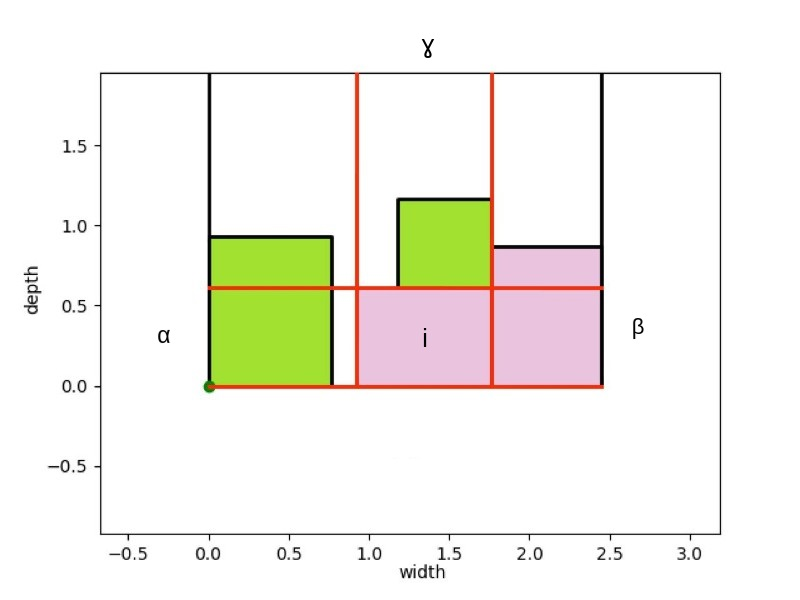
\includegraphics[width=1.\linewidth]{figures/abg_2drs}
		\caption[Vie scaricamento pacco]{Vie di scarico pacco}  
		\label{fig:abg_2drs}
	\end{minipage}%
	\begin{minipage}{.5\textwidth}
		\centering
		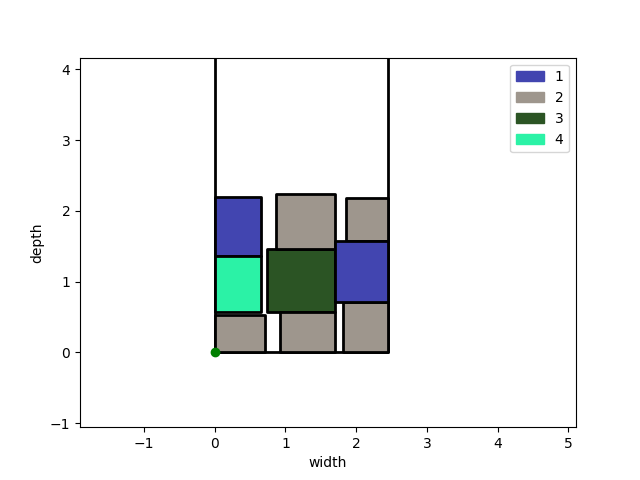
\includegraphics[width=1.\linewidth]{figures/2drs}
		\caption[Corretta sequenza di scarico]{Sequenza corretta}  
		\label{fig:2drs_abg}
	\end{minipage}
\end{figure}

Nel momento in cui l'oggetto verrà scaricato questo dovrà avere almeno una di queste vie libere affinché possa essere scaricato.
Come si può notare nella figura \ref{fig:abg_2drs}, le vie attraverso cui può essere effettuato uno scarico vengono deciso attraverso l'indice $v \in \theta = \{\alpha,\beta,\gamma\}$ che individua rispettivamente:
\begin{itemize}
	\item $v = \alpha$: via alla sinistra del pacco da cui può essere sfilato; 
	\item $v = \beta$: via alla destra del pacco da cui può essere sfilato; 
	\item $v = \gamma$: via di fronte al pacco da cui può essere sfilato; 
\end{itemize}

Il modello introduce le seguenti variabili continue positive:
\begin{itemize}
	\item la variabile continua $x_{i}$ con $i \in I$ individua la coordinata sull'asse x del vertice in basso a sinistra dell'oggetto i;
	\item la variabile continua $y_{i}$ con $i \in I$ individua la coordinata sull'asse y del vertice in basso a sinistra dell'oggetto i;
	\item la variabile continua $D$ rappresenta i metri lineari rispetto la profondità e va minimizzata.
	\item la variabile continua $\Omega_{i}$ con $i \in I$ assume il valore $d_i$ se l'oggetto è stato ruotato altrimenti $w_i$;
	\item la variabile continua $\Delta_{i}$ con $i \in I$ assume il valore $w_i$ se l'oggetto è stato ruotato altrimenti $d_i$;
\end{itemize}

Il modello introduce le seguenti variabili binarie:
\begin{itemize}
	\item la variabile binaria $l_{ij}$ con $i,j \in I$ assume il valore 1 se l'oggetto i è situato alla sinistra dell'oggetto j, altrimenti è 0;
	\item la variabile binaria $b_{ij}$ con $i,j \in I$ assume il valore 1 se l'oggetto i è situato al di sotto dell'oggetto j, altrimenti è 0.
	\item la variabile binaria $r_{i}$ con $i \in I$ assume il valore 1 se l'oggetto i è ruotato su se stesso di $90^{\circ}$, ne risulta che $w_{i}$ e $d_{i}$ sono invertiti, altrimenti è 0;
	\item la variabile binaria $\alpha_{ij}$ con $i,j \in I$ assume il valore 1 se l'oggetto i ha alla sua sinistra l'oggetto j e questo gli impedisca di essere sfilato da sinistra, altrimenti è 0;
	\item la variabile binaria $\beta_{ij}$ con $i,j \in I$ assume il valore 1 se l'oggetto i ha alla sua destra l'oggetto j e questo gli impedisca di essere sfilato da destra, altrimenti è 0;
	\item la variabile binaria $\gamma_{ij}$ con $i,j \in I$ assume il valore 1 se l'oggetto i ha davanti a se l'oggetto j e questo gli impedisca di essere sfilato centralmente, altrimenti è 0;
	\item la variabile binaria $s_{vi}$ con $i \in I$ e $v \in \theta$ assume il valore 1 se l'oggetto i ha nella direzione v almeno un oggetto che gli impedisca di essere sfilato nella rispettiva direzione, altrimenti è 0;
	\item la parametro binario $o_{ij}$ assume il valore 1 se l'oggetto i appartiene ad un ordine che deve essere scaricato prima dell'ordine a cui appartiene l'oggetto j, altrimenti è 0;
\end{itemize}

\begin{align}
	& \underset{}{\text{min D}}\\
	& \text{s.t.} & &  l_{ij} + l_{ji} + b_{ij} + b_{ji} \geq 1 & i < j && i,j \in I \label{equa30}\\
	& & & y_i - y_j + M_d b_{ij} \leq M_d - \Delta_i & & & i,j \in I \label{equa31}\\
	& & & x_i - x_j + M_w l_{ij} \leq M_w - \Omega_i & & & i,j \in I \label{equa32}\\
	& & & x_i + \Omega_i \leq W & & & i,j \in I \label{equa33}\\
	& & & y_i + \Delta_i \leq D & & & i,j \in I \label{equa34}\\
	& & & \Delta_i = d_i (1 - r_i) - w_i r_i &      &   & i,j \in I \label{equa35}\\
	& & & \Omega_i = w_i (1 - r_i) - d_i r_i &      &   & i,j \in I \label{equa36}\\
	&   &   & \alpha_{ij} \leq l_{ij}                             &   &   & i,j \in I \label{equa37} \\
	&   &   & \alpha_{ij} \leq 1 - (b_{ij} + b_{ji})              &   &   & i,j \in I \label{equa38} \\
	&   &   & \alpha_{ij} \geq l_{ij} - M_\alpha(b_{ij} + b_{ji}) &   &   & i,j \in I \label{equa39} \\
	&   &   & \beta_{ij} \leq l_{ji}                              &   &   & i,j \in I \label{equa40} \\
	&   &   & \beta_{ij} \leq 1 - (b_{ij} + b_{ji})               &   &   & i,j \in I \label{equa41} \\
	&   &   & \beta_{ij} \geq l_{ji} - M_\beta(b_{ij} + b_{ji})   &   &   & i,j \in I \label{equa42} \\
	&   &   & \gamma_{ij} \leq b_{ij}                             &   &   & i,j \in I \label{equa43} \\
	&   &   & \gamma_{ij} \leq 1 - (l_{ij} + l_{ji})              &   &   & i,j \in I \label{equa44} \\
	&   &   & \gamma_{ij} \geq b_{ij} - M_\gamma(l_{ij} + l_{ji}) &   &   & i,j \in I \label{equa45} \\
	& & & \alpha_{ij}o_{ij} \leq s_{\alpha i}  & & & i,j \in I \label{equa46}\\
	& & & \beta_{ij}o_{ij} \leq s_{\beta i}  & & & i,j \in I \label{equa47}\\
	& & & \gamma_{ij}o_{ij} \leq s_{\gamma i}  & & & i,j \in I \label{equa48}\\
	  &   &   & \sum_{v \in \theta} s_{vi} \leq 2                                     &          &   & i \in I   &   & \label{equa49} \\
	  &   &   & b_{ij}, l_{ij}, \alpha_{ij}, \beta_{ij}, \gamma_{ij}, r_i \in \{0,1\} & i \neq j &   & i,j \in I &   & \label{equa50} \\
	&             &   & x_{i}, y_{i}, w_{i}, d_{i}, \Delta_{i}, \Omega_{i} \in \mathbb{R}^{+} &          &   & i \in I  \label{equa51}\\
	&   &   & s_{vi} \in \{0,1\} &   &   & i \in I \land v\in \theta \label{equa52} 
\end{align}

\newpage
Spieghiamo ora il significato di ciascun vincolo:
\begin{itemize}
	\item il vincolo~\eqref{equa30} impone che presi due oggetti almeno uno dei due si trovi dietro o alla sinistra dell'altro;
	\item il vincolo~\eqref{equa31} dice che se $b_{ij} = 1$ allora impone che l'oggetto i si trovi dietro l'oggetto j, altrimenti il vincolo viene disattivato;
	\item il vincolo~\eqref{equa32} dice che se $l_{ij} = 1$ allora impone che l'oggetto i si trovi alla sinistra l'oggetto j, altrimenti il vincolo viene disattivato;
	\item il vincolo~\eqref{equa33} impone che dato il valore $x_i$, corrispondente alla coordinata x dell'angolo sinistro più arretrato dell'oggetto, sommandoci la larghezza $w_i$ dell'oggetto e ottenendo quindi la coordinata x dell'angolo destro più arretrato, questa sia contenuta nell'intervallo [0,W];
	\item il vincolo~\eqref{equa34} impone che dato il valore $y_i$, corrispondente alla coordinata y dell'angolo sinistro più arretrato dell'oggetto, sommandoci la profondità $d_i$ dell'oggetto e ottenendo quindi la coordinata y dell'angolo sinistro più avanzato, questa sia contenuta nell'intervallo [0,D];
	\item il vincolo~\eqref{equa35} impone che $\Delta_i$ corrisponda alla profondità corretta considerando la rotazione;
	\item il vincolo~\eqref{equa36} impone che $\Omega_i$ corrisponda alla larghezza corretta considerando la rotazione;
	\item i vincoli~\eqref{equa37},~\eqref{equa38} e~\eqref{equa39} impongono che se $l_{ij} = 1 \land t_{ij} + t_{ji} = 0 \Rightarrow \alpha_{ij} = 1$, che significa che se un oggetto i si trovi a destra di un oggetto j ma nessuno dei due sia dietro all'altro, allora l'oggetto i non potrà essere sfilato dalla sponda sinistra del camion;
	\item i vincoli~\eqref{equa40},~\eqref{equa41} e~\eqref{equa42} impongono che se $l_{ji} = 1 \land t_{ij} + t_{ji} = 0 \Rightarrow \beta_{ij} = 1$, che significa che se un oggetto i si trovi a sinistra di un oggetto j ma nessuno dei due sia dietro all'altro, allora l'oggetto i non potrà essere sfilato dalla sponda destra del camion;
	\item i vincoli~\eqref{equa43},~\eqref{equa44} e~\eqref{equa45} impongono che se $b_{ij} = 1 \land l_{ij} + l_{ji} = 0 \Rightarrow \gamma_{ij} = 1$, che significa che se un oggetto i si trovi dietro un oggetto j ma nessuno dei due sia alla sinistra dell'altro, allora l'oggetto i non potrà essere sfilato centralmente del camion;
	\item il vincolo~\eqref{equa46} impone che se $s_{1i} = 1$ allora potranno esservi dei pacchi posizionati alla sua sinistra che ne blocchino lo scarico, se $s_{1i} = 0$ allora la via dovrà essere libera permettendo così lo scarico;
	\item il vincolo~\eqref{equa47} impone che se $s_{2i} = 1$ allora potranno esservi dei pacchi posizionati alla sua destra che ne blocchino lo scarico, se $s_{2i} = 0$ allora la via dovrà essere libera permettendo così lo scarico;
	\item il vincolo~\eqref{equa48} impone che se $s_{3i} = 1$ allora potranno esservi dei pacchi posizionati davanti a sé che ne blocchino lo scarico, se $s_{3i} = 0$ allora la via dovrà essere libera permettendo così lo scarico;
	\item il vincolo~\eqref{equa49} impone che $\sum_{v \in \theta} s_{vi} \leq 2$ ossia che possano essere occupate al massimo 2 vie di scarico lasciandone libera almeno 1.
\end{itemize}

\newpage
\section{Modello 3D con rotazione e sovrapposizione}
Con questo modello, evoluzione del modello 2D con rotazione, ci si propone di introdurre la sovrapposizione degli oggetti, considerando però che alcuni oggetti potranno avere come condizione quella di non poter avere altri oggetti al di sopra.

\begin{figure}[H]
	\begin{center} 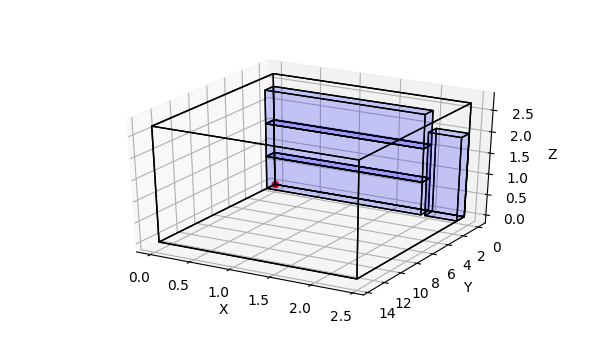
\includegraphics[scale=0.7]{figures/3d}
		\caption[Grafico con merci 3D]{Veduta 3D di alcuni pacchi.}
		\label{fig:3d_grafics}
	\end{center}
\end{figure}

Un problema non indifferente inerente questo modello viene individuato nella stabilità degli oggetti, soluzioni che riportino oggetti sopraelevati, le cui aree di base non poggino completamente sugli oggetti sottostanti sono da ritenersi non valide. Per risolvere questo problema si è deciso di optare per una semplificazione, se un oggetto i si trova sopra ad un oggetto j, allora l'area di base dell'oggetto i dovrà essere interamente appoggiata alla faccia superiore dell'oggetto j.
\newpage
Il modello 3D con rotazione e sovrapposizione introduce in più rispetto al precedente le seguenti variabili continue positive:
\begin{itemize}
	\item la variabile continua $x_{i}$ con $i \in I$ individua la coordinata sull'asse x del vertice in basso a sinistra dell'oggetto i;
	\item la variabile continua $y_{i}$ con $i \in I$ individua la coordinata sull'asse y del vertice in basso a sinistra dell'oggetto i;
	\item la variabile continua $z_{i}$ con $i \in I$ individua la coordinata sull'asse z del vertice in basso a sinistra dell'oggetto i;
	\item la variabile continua $D$ rappresenta i metri lineari rispetto la profondità e va minimizzata.
	\item la variabile continua $\Omega_{i}$ con $i \in I$ assume il valore $d_i$ se l'oggetto è stato ruotato altrimenti $w_i$;
	\item la variabile continua $\Delta_{i}$ con $i \in I$ assume il valore $w_i$ se l'oggetto è stato ruotato altrimenti $d_i$;
\end{itemize}
Introduce in più rispetto al precedente anche le seguenti variabili binarie:
\begin{itemize}
	\item la variabile binaria $l_{ij}$ con $i,j \in I$ assume il valore 1 se l'oggetto i è situato alla sinistra dell'oggetto j, altrimenti è 0;
	\item la variabile binaria $b_{ij}$ con $i,j \in I$ assume il valore 1 se l'oggetto i è situato al di sotto dell'oggetto j, altrimenti è 0.
	\item la variabile binaria $r_{i}$ con $i \in I$ assume il valore 1 se l'oggetto i è ruotato su se stesso di $90^{\circ}$, ne risulta che $w_{i}$ e $d_{i}$ sono invertiti, altrimenti è 0;
	\item la variabile binaria $t_{ij}$ assume il valore 1 se l'oggetto i ha sopra di sé l'oggetto j, altrimenti è 0;
	\item la variabile binaria $f_{ij}$ assume il valore 1 se l'oggetto i ha sopra di sé l'oggetto j e la faccia superiore dell'oggetto i è a contatto con la faccia inferiore dell'oggetto j, altrimenti è 0;
	\item la variabile binaria $k_{ij}$ con $i,j \in I$ assume il valore 1 se l'oggetto i si trova alla sinistra o/e dietro un oggetto j oppure al di sotto di esso. 
\end{itemize}
\newpage
Inoltre la variabile binaria $k_{ij}$ viene utilizzata per imporre che un oggetto possa trovarsi alla sinistra o dietro ad un altro oggetto ma non al di sotto di un altro e viceversa, imponendo ciò che segue:

\begin{align}
	& \underset{}{\text{min}}
	& & D \\
	  & \text{s.t.} &   & k_{ij} \leq l_{ij} + l_{ji} + b_{ij} + b_{ji}                                & i < j    &   & i,j \in I \label{equa53} \\
	  &             &   & 2 k_{ij} \geq l_{ij} + l_{ji} + b_{ij} + b_{ji}                              & i < j    &   & i,j \in I \label{equa54} \\
	  &             &   & 1 - k_{ij} = t_{ij} + t_{ji}                                                 & i < j    &   & i,j \in I \label{equa55} \\
	  &             &   & x_i + \Omega_i \leq W                                                        &          &   & i,j \in I \label{equa56} \\
	  &             &   & y_i + \Delta_i \leq D                                                        &          &   & i,j \in I \label{equa57} \\
	  &             &   & z_i + h_i \leq H                                                             &          &   & i \in I \label{equa58}   \\	
	  &             &   & y_i - y_j + M_d b_{ij} \leq M_d - \Delta_i                                   &          &   & i,j \in I \label{equa59} \\
	  &             &   & x_i - x_j + M_w l_{ij} \leq M_w - \Omega_i                                   &          &   & i,j \in I \label{equa60} \\
	  &             &   & z_i - z_j + M_h t_{ij} \leq M_h - h_i                                        &          &   & i,j \in I \label{equa61} \\
	  &             &   & z_i - z_j + M_h f_{ij} \geq - M_h - h_i                                      &          &   & i,j \in I \label{equa62} \\
	  &             &   & x_i - x_j \leq M_w (1-f_{ij})                                                &          &   & i,j \in I \label{equa63} \\
	  &             &   & y_i - y_j \leq M_d (1-f_{ij})                                                &          &   & i,j \in I \label{equa64} \\
	  &             &   & x_i - x_j + \Omega_i - \Omega_j \geq - Mw(1 - f_{ij})                        &          &   & i,j \in I\label{equa65}  \\
	  &             &   & y_i - y_j + \Delta_i - \Delta_j \geq - Md(1 - f_{ij})                        &          &   & i,j \in I\label{equa66}  \\
	  &             &   & f_{ij} \leq t_{ij}                                                           &          &   & i \in I \label{equa67}   \\
	  &             &   & M_h \sum_{i \in I} f_{ij} \geq z_j                                           &          &   & i \in I \label{equa68}   \\
	  &             &   & \Delta_i = d_i (1 - r_i) - w_i r_i                                           &          &   & i,j \in I \label{equa69} \\
	  &             &   & \Omega_i = w_i (1 - r_i) - d_i r_i                                           &          &   & i,j \in I \label{equa70} \\  
	  &             &   & b_{ij}, l_{ij}, t_{ij}, f_{ij}, k_{ij}, r_i \in \{0,1\}                      & i \neq j &   & i,j \in I \label{equa71} \\
	  &             &   & x_{i}, y_{i}, z_{i}, w_{i}, d_{i}, \Delta_{i}, \Omega_{i} \in \mathbb{R}^{+} &          &   & i \in I  \label{equa72}  
\end{align}
\newpage
Spieghiamo ora il significato di ciascun vincolo:
\begin{itemize}
	\item i vincoli~\eqref{equa53},~\eqref{equa54} e~\eqref{equa55} impongono che presi due oggetti uno sia dietro e/o alla sinistra dell'altro oppure sia sotto di esso;
	\item il vincolo~\eqref{equa56} impone che dato il valore $x_i$, corrispondente alla coordinata x dell'angolo sinistro più arretrato dell'oggetto, sommandoci la larghezza $w_i$ dell'oggetto e ottenendo quindi la coordinata x dell'angolo destro più arretrato, questa sia contenuta nell'intervallo [0,W];
	\item il vincolo~\eqref{equa57} impone che dato il valore $y_i$, corrispondente alla coordinata y dell'angolo sinistro più arretrato dell'oggetto, sommandoci la profondità $d_i$ dell'oggetto e ottenendo quindi la coordinata y dell'angolo sinistro più avanzato, questa sia contenuta nell'intervallo [0,D];
	\item il vincolo~\eqref{equa58} impone che dato il valore $z_i$, corrispondente alla coordinata z dell'angolo sinistro più arretrato dell'oggetto, sommandoci l'altezza $h_i$ dell'oggetto e ottenendo quindi la coordinata z dell'angolo sinistro più in alto, questa sia contenuta nell'intervallo [0,H];
	\item il vincolo~\eqref{equa59} dice che se $b_{ij} = 1$ allora impone che l'oggetto i si trovi dietro l'oggetto j, altrimenti il vincolo viene disattivato;
	\item il vincolo~\eqref{equa60} dice che se $l_{ij} = 1$ allora impone che l'oggetto i si trovi alla sinistra l'oggetto j, altrimenti il vincolo viene disattivato;
	\item il vincolo~\eqref{equa61} dice che se $t_{ij} = 1$ allora impone che l'oggetto i si trovi al di sotto dell'oggetto j, altrimenti il vincolo viene disattivato;
	\item il vincolo~\eqref{equa62} dice che se $f_{ij} = 1$ allora impone che l'oggetto i si trovi al di sotto dell'oggetto j e a contatto con lo stesso, altrimenti il vincolo viene disattivato;
	\item i vincoli~\eqref{equa63} e~\eqref{equa64} impongono che se un oggetto i è sotto e a contatto con un oggetto j, allora la coordinata dell'angolo più vicino all'origine dovrà trovarsi all'interno del piano individuato dalla base superiore dell'oggetto i;
	\item i vincoli~\eqref{equa65} e~\eqref{equa66} impongono che se un oggetto i è sotto e a contatto con un oggetto j, allora la coordinata dell'angolo più lontano all'origine dovrà trovarsi all'interno del piano individuato dalla base superiore dell'oggetto i;
	\item il vincolo~\eqref{equa67} impone che un oggetto i possa essere al di sotto e a contatto con un oggetto j solo se l'oggetto i è al di sotto dell'oggetto j;
	\item il vincolo~\eqref{equa68} impone che tutti gli oggetti i che non abbiano al di sotto di sé nessun oggetto debbano avere coordinata $z_i=0$
	\item il vincolo~\eqref{equa69} impone che $\Delta_i$ corrisponda alla profondità corretta considerando la rotazione;
	\item il vincolo~\eqref{equa70} impone che $\Omega_i$ corrisponda alla larghezza corretta considerando la rotazione;
\end{itemize}

